\documentclass[landscape]{jhuslides3C}
\usepackage{url}
\usepackage{amsmath}
\usepackage{graphicx}
\usepackage{color}
\usepackage{colortbl}
\usepackage{epic,ecltree}
%\usepackage{bar}
\usepackage{array}% http://ctan.org/pkg/array
\usepackage{qtree}
\usepackage{eclbip}
\usepackage{fancybox}
\usepackage{pause} % java -jar ~/Code/statmt/bin/pp4p.jar mtsummit09-talk.pdf mtsummit09-talk.view.pdf
\usepackage[absolute]{textpos}
\pdfoptionpdfminorversion 3
\usepackage{palatino}
\usepackage{tikz}
%\usepackage{tikz-qtree}
\usetikzlibrary{calc,matrix}
\usepackage{algorithmic}
\usepackage{algorithm}
\usepackage{amssymb,latexsym} % for \blacklozenge
\renewcommand{\algorithmicrequire}{\textbf{Input:}}
\renewcommand{\algorithmicensure}{\textbf{Output:}}
\renewcommand{\algorithmiccomment}[1]{// {\em #1}}
\usepackage{multicol}
\usepackage{wasysym} % smileys
\renewcommand*\ttdefault{txtt} % 20% tighter than courier
\usepackage{pgfplots}

\usetikzlibrary{positioning,shadows,arrows}

\definecolor{lightblue}{rgb}{.8,.8,1}
\definecolor{mediumlightblue}{rgb}{.5,.5,1}
\definecolor{lightyellow}{rgb}{1,1,.5}
\definecolor{lightorange}{rgb}{1,.9,.7}
\definecolor{darkorange}{rgb}{1,.75,.2}
\definecolor{sortadarkorange}{rgb}{.8,.5,.1}
\definecolor{verydarkorange}{rgb}{.5,.3,0}
\definecolor{darkblue}{rgb}{0,0,0.8}
\definecolor{verydarkgreen}{rgb}{0,0.4,0}
\definecolor{darkgreen}{rgb}{0,0.8,0}
\definecolor{darkred}{rgb}{0.8,0,0}
\definecolor{verydarkred}{rgb}{0.6,0,0}
\definecolor{lightgreen}{rgb}{.8,1,.8}
\definecolor{lightred}{rgb}{1,.8,.8}
\definecolor{darkgrey}{rgb}{0.5,0.5,0.5}
\definecolor{purple}{rgb}{0.6,0,0.6}
\definecolor{red}{rgb}{1,0,0}
\definecolor{orange}{rgb}{.8,.6,0}
\definecolor{cyan}{rgb}{0,.6,.6}
\definecolor{reddishgreen}{rgb}{0.4,0.6,0}

\newcommand{\newconcept}[1]{\textcolor{blue}{\bf #1}}
\newcommand{\example}[1]{\textcolor{darkblue}{\em #1}}
\newcommand{\important}[1]{\textcolor{darkblue}{\em #1}}
\newcommand{\concept}[1]{\textcolor{darkblue}{\em #1}}
\newcommand{\maths}[1]{\textcolor{purple}{#1}}
\newcommand{\reference}[1]{\vspace{-2mm}\begin{flushright}\textcolor{purple}{\tiny [from #1]}\end{flushright}\vspace{-7mm}}
\renewcommand{\url}[1]{\textcolor{verydarkred}{\tt #1}}

\newcommand{\highlightbox}[6]{\begin{textblock}{#3}(#1,#2) \colorbox{#4}{\textcolor{#5}{\begin{minipage}{#3in} #6 \end{minipage} }} \end{textblock}}
\newcommand{\backgroundbox}[5]{\highlightbox{#1}{#2}{#3}{#5}{black}{\vspace{#4in}\hspace{#3in}}}
\newcommand{\currenttopic}[1]{\colorbox{lightyellow}{\textcolor{black}{\bf #1}}}

\newcommand{\littlecode}[1]{\colorbox{gray}{\textcolor{black}{\small \tt #1}}}
\newcommand{\highlight}[1]{\colorbox{lightyellow}{#1}}
\newcommand{\highlightOrange}[1]{\colorbox{lightorange}{#1}}
\newcommand{\highlightGreen}[1]{\colorbox{lightgreen}{#1}}
\newcommand{\highlightBlue}[1]{\colorbox{lightblue}{#1}}

%%%%%%%%%%%%%%%%%%%%%%%%%%%%%%%%%%%%%%%%%%%%%%%%%%%%%%%%%%%%%%%%%%%%%%%%%%%%

\begin{document} \rm
\title[Machine Translation: Current Challenges]{Current Challenges}
\author[Philipp Koehn]{Philipp Koehn}
\date{5 November 2020}
\maketitle

%%%%%%%%%%%%%%%%%%%%%%%%%%%%%%%%%%%%%%%%%%%%%%%%%%%%%%%%%%%%%%%%%%%%%%%%%%%%

\slide{WMT 2016}
\vfill
\begin{center}
\includegraphics[scale=0.75]{wmt16-english-german-labeled.pdf}\\[3mm]
(in 2017 barely any statistical machine translation submissions)
\end{center}
\vfill


%%%%%%%%%%%%%%%%%%%%%%%%%%%%%%%%%%%%%%%%%%%%%%%%%%%%%%%%%%%%%%%%%%%%%%%%%%%%

\slide{2017: Google: "Near Human Quality"}
\vfill
\begin{center}
\includegraphics[scale=0.8]{google-near-human.png}
\end{center}
\vfill

%%%%%%%%%%%%%%%%%%%%%%%%%%%%%%%%%%%%%%%%%%%%%%%%%%%%%%%%%%%%%%%%%%%%%%%%%%%%

\slide{2018: More Hype}
\vfill
\begin{center}
\includegraphics[scale=1.15]{ms-zh-parity.png}\\[1cm]
\includegraphics[scale=0.85]{sdl-cracks-russian.png}\\
{\em \small ``90\% of the system's output labelled as perfect by professional Russian-English translators''}
\end{center}
\vfill

%%%%%%%%%%%%%%%%%%%%%%%%%%%%%%%%%%%%%%%%%%%%%%%%%%%%%%%%%%%%%%%%%%%%%%%%%%%%

\slide{Just Better Fluency?}
\vfill
\begin{center}
\includegraphics[width=25cm]{nmt-adequacy-fluency-wmt16.png}\\[1cm]
(from: Sennrich and Haddow, 2017)
\end{center}
\vfill

%%%%%%%%%%%%%%%%%%%%%%%%%%%%%%%%%%%%%%%%%%%%%%%%%%%%%%%%%%%%%%%%%%%%%%%%%%%%

\slide{Challenges}
\vfill
\begin{itemize}
%\item Last lectures: architecture of attentional sequence-to-sequence neural model
\item Lack of training data
\item Domain mismatch
\item Rare words
\item Word alignment
\item Beam search
\item Noise
\item Control over output
\item Interpretability
\end{itemize}
\vfill

%%%%%%%%%%%%%%%%%%%%%%%%%%%%%%%%%%%%%%%%%%%%%%%%%%%%%%%%%%%%%%%%%%%%%%%%%%%%

\slide{}
\vfill
\begin{center}
{\huge lack of training data}
\end{center}
\vfill

%%%%%%%%%%%%%%%%%%%%%%%%%%%%%%%%%%%%%%%%%%%%%%%%%%%%%%%%%%%%%%%%%%%%%%%%%%%%

\slide{Amount of Training Data}
\begin{center}
\small
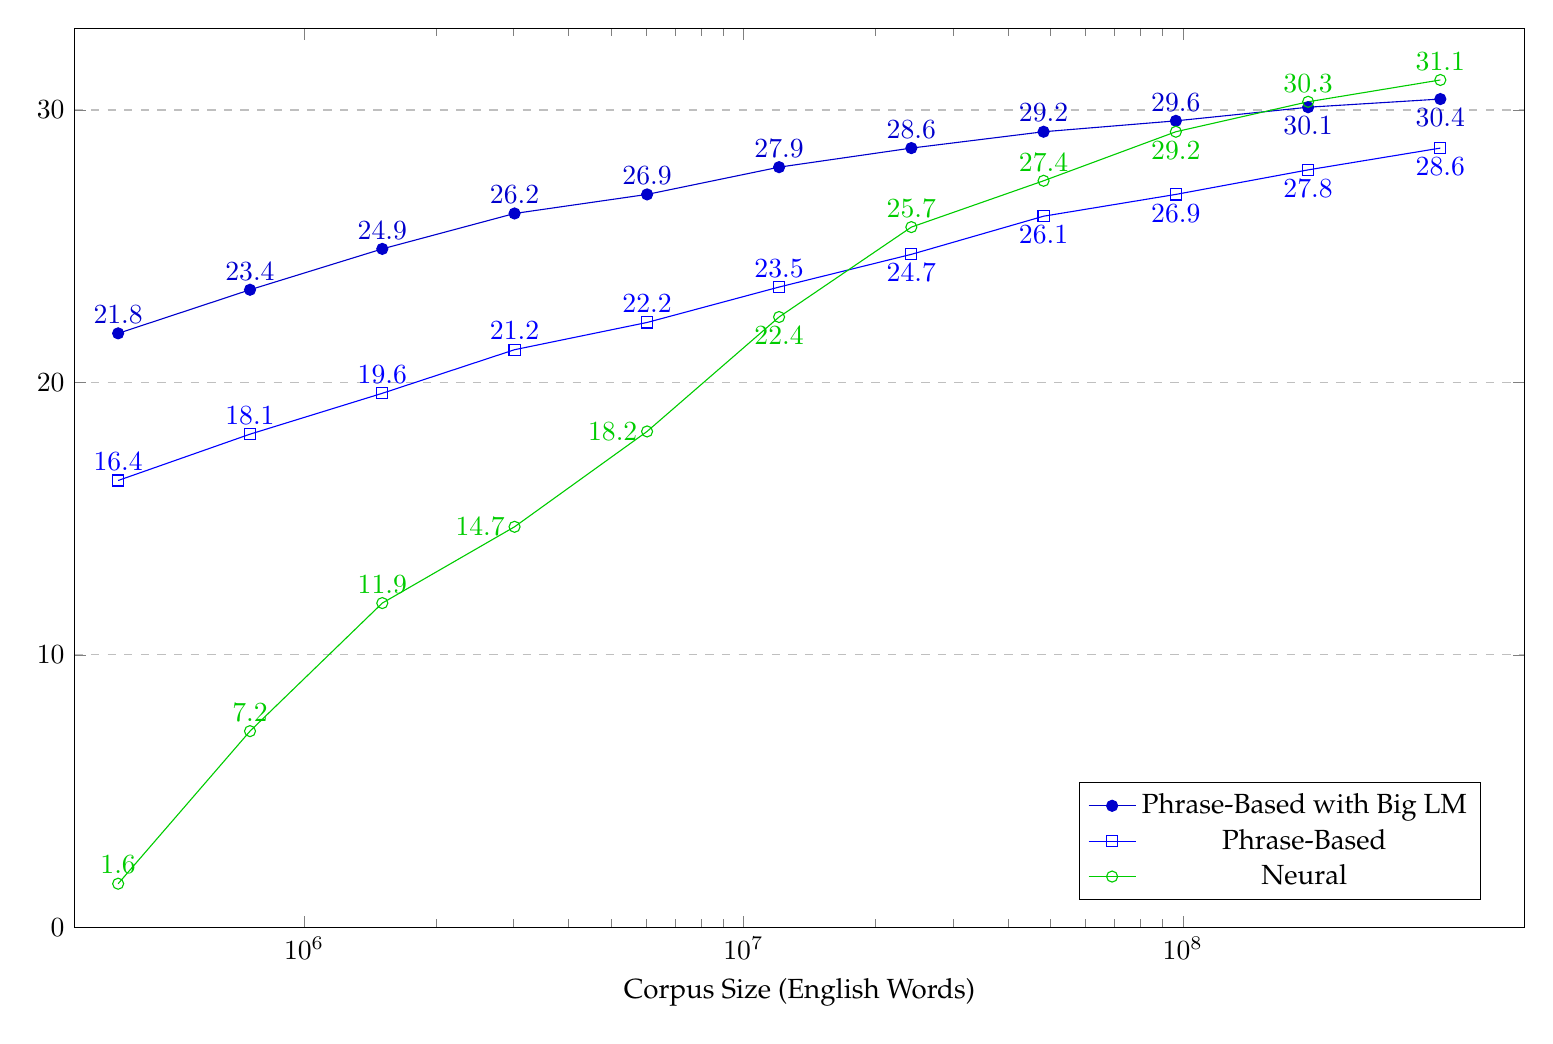
\begin{tikzpicture}
\begin{semilogxaxis}[
    xlabel={Corpus Size (English Words)},
    %ylabel={BLEU},
    width=20cm,
    height=13cm,
    xmin=300000, xmax=600000000,
    ymin=0, ymax=33,
    xtick={1000000,10000000,100000000},
    ytick={0,10,20,30},
    legend pos=south east,
    ymajorgrids=true,
    grid style=dashed,
]
 
%%% Phrase-Based with Big LM
\addplot[
    color=darkblue,
    mark=*,
    nodes near coords,
    nodes near coords align={\thealign},
    visualization depends on={value \thisrow{ALIGN} \as \thealign},
    ]
    table[x=X, y=Y]{
        X    Y ALIGN SIZE 
   377411 21.8 south 1024 
   753253 23.4 south  512  
  1506597 24.9 south  256  
  3013217 26.2 south  128  
  6035176 26.9 south   64  
 12053137 27.9 south   32  
 24107029 28.6 south   16  
 48204905 29.2 south    8  
 96433893 29.6 south    4  
192873315 30.1 north    2 
385703602 30.4 north    1
    };
    \addlegendentry{Phrase-Based with Big LM}

%%% Phrase-Based
\addplot[
    color=blue,
    mark=square,
    nodes near coords,
    %every node near coord/.append style={anchor={north}}
    nodes near coords align={\thealign},
    visualization depends on={value \thisrow{ALIGN} \as \thealign},
    ]
    table[x=X, y=Y]{
        X    Y ALIGN SIZE 
   377411 16.4 south 1024 
   753253 18.1 south  512  
  1506597 19.6 south  256  
  3013217 21.2 south  128  
  6035176 22.2 south   64  
 12053137 23.5 south   32  
 24107029 24.7 north   16  
 48204905 26.1 north    8  
 96433893 26.9 north    4  
192873315 27.8 north    2 
385703602 28.6 north    1
    };
    \addlegendentry{Phrase-Based}
    
    
%%% Neural
\addplot[
    color=darkgreen,
    mark=o,
    nodes near coords,
    nodes near coords align={\thealign},
    visualization depends on={value \thisrow{ALIGN} \as \thealign},
    ]
    table[x=X, y=Y]{
        X    Y ALIGN SIZE 
   377411  1.6 south 1024 
   753253  7.2 south  512  
  1506597 11.9 south  256  
  3013217 14.7 east   128  
  6035176 18.2 east    64  
 12053137 22.4 north   32  
 24107029 25.7 south   16  
 48204905 27.4 south    8  
 96433893 29.2 north    4  
192873315 30.3 south    2 
385703602 31.1 south    1
    };
    \addlegendentry{Neural}
\end{semilogxaxis}
\end{tikzpicture}
\end{center}

English-Spanish systems trained on 0.4 million to 385.7 million words

%%%%%%%%%%%%%%%%%%%%%%%%%%%%%%%%%%%%%%%%%%%%%%%%%%%%%%%%%%%%%%%%%%%%%%%%%%%%

\slide{Translation Examples}
\vfill
\begin{tabular}{c|p{22cm}}
Source & A Republican strategy to counter the re-election of Obama\\\hline\hline
$\frac{1}{1024}$ & Un {\'o}rgano de coordinaci{\'o}n para el anuncio de libre determinaci{\'o}n\\ \hline
$\frac{1}{512}$ & Lista de una estrategia para luchar contra la elecci{\'o}n de hojas de Ohio\\\hline
$\frac{1}{256}$ & Explosi{\'o}n realiza una estrategia divisiva de luchar contra las elecciones de autor\\\hline
$\frac{1}{128}$ & Una estrategia republicana para la eliminaci{\'o}n de la reelecci{\'o}n de Obama\\\hline
$\frac{1}{64}$ & Estrategia siria para contrarrestar la reelecci{\'o}n del Obama .\\\hline
$\frac{1}{32}+$ & Una estrategia republicana para contrarrestar la reelecci{\'o}n de Obama\\
\end{tabular}
\vfill

%%%%%%%%%%%%%%%%%%%%%%%%%%%%%%%%%%%%%%%%%%%%%%%%%%%%%%%%%%%%%%%%%%%%%%%%%%%%

\slide{}
\vfill
\begin{center}
{\huge domain mismatch}
\end{center}
\vfill

%%%%%%%%%%%%%%%%%%%%%%%%%%%%%%%%%%%%%%%%%%%%%%%%%%%%%%%%%%%%%%%%%%%%%%%%%%%%

\slide{Domain Mismatch}
\vfill
\newcommand{\barchart}[2]{\begin{tikzpicture}[scale=0.02]
\fill[green] (0,0) rectangle (55,#1);
\fill[blue] (60,0) rectangle (115,#2);
\draw (27.5,0) node[anchor=north] {#1};
\draw (87.5,0) node[anchor=north] {#2};
\end{tikzpicture}}
\newcommand{\rowlabel}[1]{\begin{tikzpicture}[scale=0.02]\fill[white] (0,0) rectangle (2,2);\draw (1,0) node[anchor=north] {\bf #1}; \end{tikzpicture}}
\begin{center}
\begin{tabular}{l|c|c|c|c|c}
\bf System $\downarrow$ & \bf Law & \bf Medical& \bf IT& \bf Koran& \bf Subtitles \\ \hline \hline
\rowlabel{All Data} & \barchart{30.5}{32.8} & \barchart{45.1}{42.2} & \barchart{35.3}{44.7} & \barchart{17.9}{17.9} & \barchart{26.4}{20.8}\\\hline \hline
\rowlabel{Law} & \cellcolor{lightgray}\barchart{31.1}{34.4} & \barchart{12.1}{18.2} & \barchart{3.5}{6.9} & \barchart{1.3}{2.2} & \barchart{2.8}{6.0}\\\hline
\rowlabel{Medical} & \barchart{3.9}{10.2} & \cellcolor{lightgray}\barchart{39.4}{43.5} & \barchart{2.0}{8.5} & \barchart{0.6}{2.0} & \barchart{1.4}{5.8}\\\hline
\rowlabel{IT} & \barchart{1.9}{3.7} & \barchart{6.5}{5.3} & \cellcolor{lightgray}\barchart{42.1}{39.8} & \barchart{1.8}{1.6} & \barchart{3.9}{4.7}\\\hline
\rowlabel{Koran} & \barchart{0.4}{1.8} & \barchart{0.0}{2.1} & \barchart{0.0}{2.3} & \cellcolor{lightgray}\barchart{15.9}{18.8} & \barchart{1.0}{5.5}\\\hline
\rowlabel{Subtitles} & \barchart{7.0}{9.9} & \barchart{9.3}{17.8} & \barchart{9.2}{13.6} & \barchart{9.0}{8.4} & \cellcolor{lightgray}\barchart{25.9}{22.1}\\\hline
\end{tabular}
\end{center}
\vfill

%%%%%%%%%%%%%%%%%%%%%%%%%%%%%%%%%%%%%%%%%%%%%%%%%%%%%%%%%%%%%%%%%%%%%%%%%%%%

\slide{Translation Examples}
\vfill
\begin{tabular}{l|p{22cm}}
Source & Schaue um dich herum.\\ \hline
Ref. & Look around you. \\ \hline \hline
All & NMT: Look around you.\\
& SMT: Look around you.\\\hline
Law & NMT: Sughum gravecorn.\\
& SMT: In order to implement dich Schaue .\\\hline
Medical & NMT: EMEA / MB / 049 / 01-EN-Final Work progamme for 2002\\
& SMT: Schaue by dich around .\\\hline
IT & NMT: Switches to paused.\\
& SMT: To Schaue by itself . \textbackslash t \textbackslash t\\\hline
Koran & NMT: Take heed of your own souls.\\
& SMT: And you see. \\\hline
Subtitles & NMT: Look around you.\\
& SMT: Look around you .
\end{tabular}
\vfill


%%%%%%%%%%%%%%%%%%%%%%%%%%%%%%%%%%%%%%%%%%%%%%%%%%%%%%%%%%%%%%%%%%%%%%%%%%%%

\slide{}
\vfill
\begin{center}
{\huge rare words}
\end{center}
\vfill

%%%%%%%%%%%%%%%%%%%%%%%%%%%%%%%%%%%%%%%%%%%%%%%%%%%%%%%%%%%%%%%%%%%%%%%%%%%%

\slide{Rare Words}
\vfill
\begin{itemize}
\item More frequent in training $\rightarrow$ more likely to get right in test
\item Let's measure this\pause
\item One problem
\begin{itemize}\itemsep 2mm
\item frequency measured for input words
\item translation correctness measured for output words
\end{itemize}
\end{itemize}
\vfill

%%%%%%%%%%%%%%%%%%%%%%%%%%%%%%%%%%%%%%%%%%%%%%%%%%%%%%%%%%%%%%%%%%%%%%%%%%%%

\slide{Translation Accuracy for Input Words}
\vfill
\begin{itemize}
\item Generate word alignment between input and output words
\item Look up count of input word in training
\item Link to output word via word alignment
\item Check if it is also in the reference translation\pause
\item A lot of tedious special cases
\begin{itemize}
\item one-to-many alignment, only some output words in reference
\item input word not aligned to any target word
\item many-to-one alignment
\item output word occurs multiple time in output or reference sentence
\end{itemize}
\end{itemize}
\vfill

%%%%%%%%%%%%%%%%%%%%%%%%%%%%%%%%%%%%%%%%%%%%%%%%%%%%%%%%%%%%%%%%%%%%%%%%%%%%

\slide{Count vs. Accuracy}
\vfill
\begin{center}
accuracy

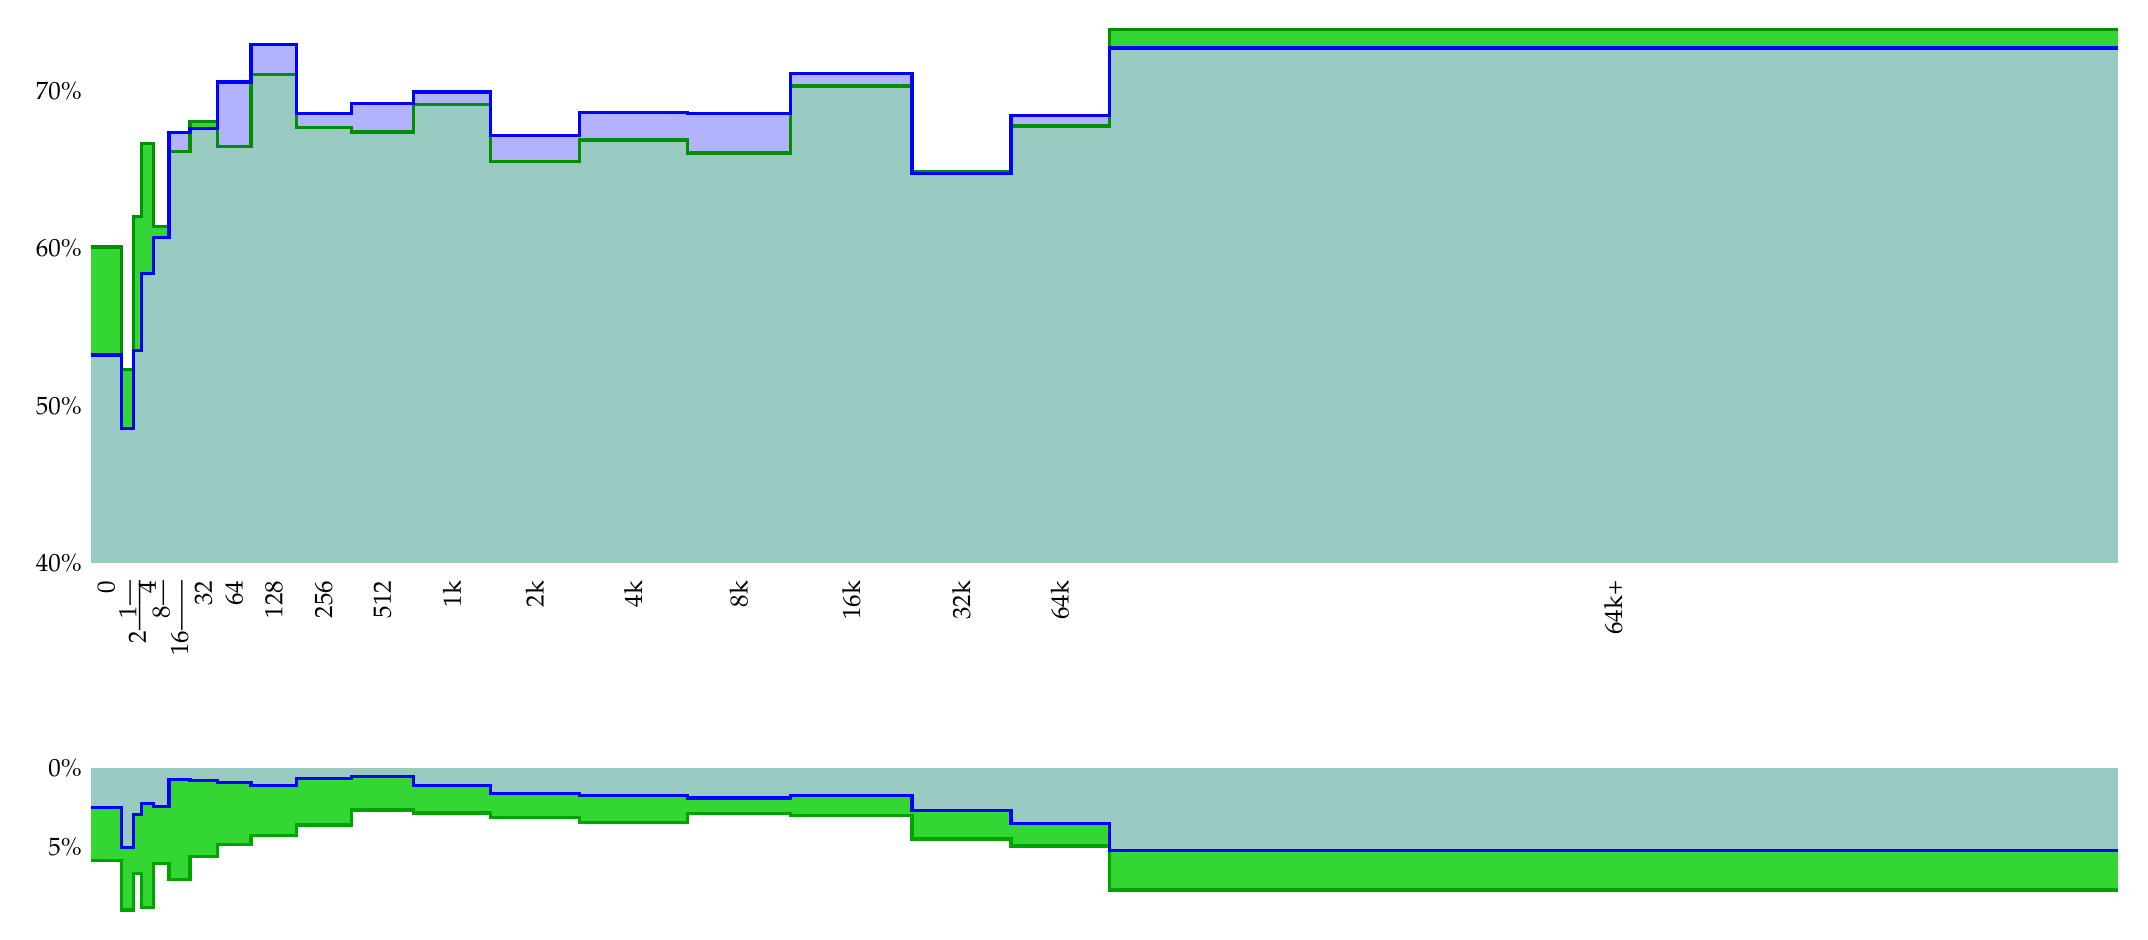
\begin{tikzpicture}[scale=20]\small
\small
\fill[darkgreen!60!blue!40!white] (0,0) rectangle (0.01978,0.13222997611);
\fill[darkgreen!80!white] (0,0.13222997611) rectangle (0.01978,0.200737232692);
\fill[darkgreen!60!blue!40!white] (0.01978,0) rectangle (0.02732,0.085529879804);
\fill[darkgreen!80!white] (0.01978,0.085529879804) rectangle (0.02732,0.122895132079);
\fill[darkgreen!60!blue!40!white] (0.02732,0) rectangle (0.03208,0.134848484848);
\fill[darkgreen!80!white] (0.02732,0.134848484848) rectangle (0.03208,0.22012012012);
\fill[darkgreen!60!blue!40!white] (0.03208,0) rectangle (0.03996,0.183976499691);
\fill[darkgreen!80!white] (0.03208,0.183976499691) rectangle (0.03996,0.266620241411);
\fill[darkgreen!60!blue!40!white] (0.03996,0) rectangle (0.04982,0.206659106659);
\fill[darkgreen!80!white] (0.03996,0.206659106659) rectangle (0.04982,0.213786897048);
\fill[darkgreen!60!blue!40!white] (0.04982,0) rectangle (0.06308,0.261277958153);
\fill[blue!30!white] (0.04982,0.261277958153) rectangle (0.06308,0.273362039851);
\fill[darkgreen!60!blue!40!white] (0.06308,0) rectangle (0.08052,0.276048883757);
\fill[darkgreen!80!white] (0.06308,0.276048883757) rectangle (0.08052,0.280376670717);
\fill[darkgreen!60!blue!40!white] (0.08052,0) rectangle (0.10182,0.264346824613);
\fill[blue!30!white] (0.08052,0.264346824613) rectangle (0.10182,0.305581885203);
\fill[darkgreen!60!blue!40!white] (0.10182,0) rectangle (0.13082,0.310074447646);
\fill[blue!30!white] (0.10182,0.310074447646) rectangle (0.13082,0.329311947931);
\fill[darkgreen!60!blue!40!white] (0.13082,0) rectangle (0.16546,0.276802476533);
\fill[blue!30!white] (0.13082,0.276802476533) rectangle (0.16546,0.285416666667);
\fill[darkgreen!60!blue!40!white] (0.16546,0) rectangle (0.20522,0.273818752307);
\fill[blue!30!white] (0.16546,0.273818752307) rectangle (0.20522,0.29184370258);
\fill[darkgreen!60!blue!40!white] (0.20522,0) rectangle (0.25392,0.291074700493);
\fill[blue!30!white] (0.20522,0.291074700493) rectangle (0.25392,0.299135981912);
\fill[darkgreen!60!blue!40!white] (0.25392,0) rectangle (0.31034,0.254877379209);
\fill[blue!30!white] (0.25392,0.254877379209) rectangle (0.31034,0.271422994423);
\fill[darkgreen!60!blue!40!white] (0.31034,0) rectangle (0.37882,0.268617414692);
\fill[blue!30!white] (0.31034,0.268617414692) rectangle (0.37882,0.28606817281);
\fill[darkgreen!60!blue!40!white] (0.37882,0) rectangle (0.4446,0.260455162334);
\fill[blue!30!white] (0.37882,0.260455162334) rectangle (0.4446,0.28561427981);
\fill[darkgreen!60!blue!40!white] (0.4446,0) rectangle (0.52154,0.303029490617);
\fill[blue!30!white] (0.4446,0.303029490617) rectangle (0.52154,0.311076563465);
\fill[darkgreen!60!blue!40!white] (0.52154,0) rectangle (0.58434,0.24728314239);
\fill[darkgreen!80!white] (0.52154,0.24728314239) rectangle (0.58434,0.248513824031);
\fill[darkgreen!60!blue!40!white] (0.58434,0) rectangle (0.6468,0.277647686433);
\fill[blue!30!white] (0.58434,0.277647686433) rectangle (0.6468,0.284259478767);
\fill[darkgreen!60!blue!40!white] (0.6468,0) rectangle (1.2875,0.327062571024);
\fill[darkgreen!80!white] (0.6468,0.327062571024) rectangle (1.2875,0.338964673808);
\draw[darkgreen!70!black,very thick]  (0,0.200737232692) --  (0.01978,0.200737232692) --  (0.01978,0.122895132079) --  (0.02732,0.122895132079) --  (0.02732,0.22012012012) --  (0.03208,0.22012012012) --  (0.03208,0.266620241411) --  (0.03996,0.266620241411) --  (0.03996,0.213786897048) --  (0.04982,0.213786897048) --  (0.04982,0.261277958153) --  (0.06308,0.261277958153) --  (0.06308,0.280376670717) --  (0.08052,0.280376670717) --  (0.08052,0.264346824613) --  (0.10182,0.264346824613) --  (0.10182,0.310074447646) --  (0.13082,0.310074447646) --  (0.13082,0.276802476533) --  (0.16546,0.276802476533) --  (0.16546,0.273818752307) --  (0.20522,0.273818752307) --  (0.20522,0.291074700493) --  (0.25392,0.291074700493) --  (0.25392,0.254877379209) --  (0.31034,0.254877379209) --  (0.31034,0.268617414692) --  (0.37882,0.268617414692) --  (0.37882,0.260455162334) --  (0.4446,0.260455162334) --  (0.4446,0.303029490617) --  (0.52154,0.303029490617) --  (0.52154,0.248513824031) --  (0.58434,0.248513824031) --  (0.58434,0.277647686433) --  (0.6468,0.277647686433) --  (0.6468,0.338964673808) --  (1.2875,0.338964673808);
\draw[blue,very thick]  (0,0.13222997611) --  (0.01978,0.13222997611) --  (0.01978,0.085529879804) --  (0.02732,0.085529879804) --  (0.02732,0.134848484848) --  (0.03208,0.134848484848) --  (0.03208,0.183976499691) --  (0.03996,0.183976499691) --  (0.03996,0.206659106659) --  (0.04982,0.206659106659) --  (0.04982,0.273362039851) --  (0.06308,0.273362039851) --  (0.06308,0.276048883757) --  (0.08052,0.276048883757) --  (0.08052,0.305581885203) --  (0.10182,0.305581885203) --  (0.10182,0.329311947931) --  (0.13082,0.329311947931) --  (0.13082,0.285416666667) --  (0.16546,0.285416666667) --  (0.16546,0.29184370258) --  (0.20522,0.29184370258) --  (0.20522,0.299135981912) --  (0.25392,0.299135981912) --  (0.25392,0.271422994423) --  (0.31034,0.271422994423) --  (0.31034,0.28606817281) --  (0.37882,0.28606817281) --  (0.37882,0.28561427981) --  (0.4446,0.28561427981) --  (0.4446,0.311076563465) --  (0.52154,0.311076563465) --  (0.52154,0.24728314239) --  (0.58434,0.24728314239) --  (0.58434,0.284259478767) --  (0.6468,0.284259478767) --  (0.6468,0.327062571024) --  (1.2875,0.327062571024);

\node[label=below:\rotatebox{90}{\small 0}] at (0.00989,0) {};
\node[label=below:\rotatebox{90}{\small 1---}] at (0.02355,0) {};
\node[label=below:\rotatebox{90}{\small 2------}] at (0.0297,0) {};
\node[label=below:\rotatebox{90}{\small 4}] at (0.03602,0) {};
\node[label=below:\rotatebox{90}{8---}] at (0.04489,0) {};
\node[label=below:\rotatebox{90}{16------}] at (0.05645,0) {};
\node[label=below:\rotatebox{90}{32}] at (0.0718,0) {};
\node[label=below:\rotatebox{90}{64}] at (0.09117,0) {};
\node[label=below:\rotatebox{90}{128}] at (0.11632,0) {};
\node[label=below:\rotatebox{90}{256}] at (0.14814,0) {};
\node[label=below:\rotatebox{90}{512}] at (0.18534,0) {};
\node[label=below:\rotatebox{90}{1k}] at (0.22957,0) {};
\node[label=below:\rotatebox{90}{2k}] at (0.28213,0) {};
\node[label=below:\rotatebox{90}{4k}] at (0.34458,0) {};
\node[label=below:\rotatebox{90}{8k}] at (0.41171,0) {};
\node[label=below:\rotatebox{90}{16k}] at (0.48307,0) {};
\node[label=below:\rotatebox{90}{32k}] at (0.55294,0) {};
\node[label=below:\rotatebox{90}{64k}] at (0.61557,0) {};
\node[label=below:\rotatebox{90}{\small 64k+}] at (0.96715,0) {};

\draw (0,0) node[anchor=east] {40\%};
\draw (0,0.1) node[anchor=east] {50\%};
\draw (0,0.2) node[anchor=east] {60\%};
\draw (0,0.3) node[anchor=east] {70\%};
\draw (0,-0.13) node[anchor=east] {0\%};
\draw (0,-0.18) node[anchor=east] {5\%};

\fill[darkgreen!60!blue!40!white] (0,-0.13) rectangle (0.01978,-0.155278058645096);
\fill[darkgreen!80!white] (0,-0.155278058645096) rectangle (0.01978,-0.188645096056623);
\fill[darkgreen!60!blue!40!white] (0.01978,-0.13) rectangle (0.02732,-0.180397877984085);
\fill[darkgreen!80!white] (0.01978,-0.180397877984085) rectangle (0.02732,-0.220185676392573);
\fill[darkgreen!60!blue!40!white] (0.02732,-0.13) rectangle (0.03208,-0.159411764705882);
\fill[darkgreen!80!white] (0.02732,-0.159411764705882) rectangle (0.03208,-0.197226890756303);
\fill[darkgreen!60!blue!40!white] (0.03208,-0.13) rectangle (0.03996,-0.152842639593909);
\fill[darkgreen!80!white] (0.03208,-0.152842639593909) rectangle (0.03996,-0.218832487309645);
\fill[darkgreen!60!blue!40!white] (0.03996,-0.13) rectangle (0.04982,-0.154340770791075);
\fill[darkgreen!80!white] (0.03996,-0.154340770791075) rectangle (0.04982,-0.190851926977688);
\fill[darkgreen!60!blue!40!white] (0.04982,-0.13) rectangle (0.06308,-0.137541478129713);
\fill[darkgreen!80!white] (0.04982,-0.137541478129713) rectangle (0.06308,-0.200889894419306);
\fill[darkgreen!60!blue!40!white] (0.06308,-0.13) rectangle (0.08052,-0.13802752293578);
\fill[darkgreen!80!white] (0.06308,-0.13802752293578) rectangle (0.08052,-0.186192660550459);
\fill[darkgreen!60!blue!40!white] (0.08052,-0.13) rectangle (0.10182,-0.139389671361502);
\fill[darkgreen!80!white] (0.08052,-0.139389671361502) rectangle (0.10182,-0.178826291079812);
\fill[darkgreen!60!blue!40!white] (0.10182,-0.13) rectangle (0.13082,-0.141034482758621);
\fill[darkgreen!80!white] (0.10182,-0.141034482758621) rectangle (0.13082,-0.172758620689655);
\fill[darkgreen!60!blue!40!white] (0.13082,-0.13) rectangle (0.16546,-0.136928406466513);
\fill[darkgreen!80!white] (0.13082,-0.136928406466513) rectangle (0.16546,-0.166374133949192);
\fill[darkgreen!60!blue!40!white] (0.16546,-0.13) rectangle (0.20522,-0.135533199195171);
\fill[darkgreen!80!white] (0.16546,-0.135533199195171) rectangle (0.20522,-0.156659959758551);
\fill[darkgreen!60!blue!40!white] (0.20522,-0.13) rectangle (0.25392,-0.141088295687885);
\fill[darkgreen!80!white] (0.20522,-0.141088295687885) rectangle (0.25392,-0.158747433264887);
\fill[darkgreen!60!blue!40!white] (0.25392,-0.13) rectangle (0.31034,-0.14630627437079);
\fill[darkgreen!80!white] (0.25392,-0.14630627437079) rectangle (0.31034,-0.161549096065225);
\fill[darkgreen!60!blue!40!white] (0.31034,-0.13) rectangle (0.37882,-0.147523364485981);
\fill[darkgreen!80!white] (0.31034,-0.147523364485981) rectangle (0.37882,-0.164754672897196);
\fill[darkgreen!60!blue!40!white] (0.37882,-0.13) rectangle (0.4446,-0.149154758285193);
\fill[darkgreen!80!white] (0.37882,-0.149154758285193) rectangle (0.4446,-0.159188203101247);
\fill[darkgreen!60!blue!40!white] (0.4446,-0.13) rectangle (0.52154,-0.147676111255524);
\fill[darkgreen!80!white] (0.4446,-0.147676111255524) rectangle (0.52154,-0.160413309072004);
\fill[darkgreen!60!blue!40!white] (0.52154,-0.13) rectangle (0.58434,-0.157070063694268);
\fill[darkgreen!80!white] (0.52154,-0.157070063694268) rectangle (0.58434,-0.175222929936306);
\fill[darkgreen!60!blue!40!white] (0.58434,-0.13) rectangle (0.6468,-0.165222542427153);
\fill[darkgreen!80!white] (0.58434,-0.165222542427153) rectangle (0.6468,-0.179631764329171);
\fill[darkgreen!60!blue!40!white] (0.6468,-0.13) rectangle (1.2875,-0.182505072576869);
\fill[darkgreen!80!white] (0.6468,-0.182505072576869) rectangle (1.2875,-0.20747775870142);

\draw[darkgreen!80!black,very thick]  (0,-0.188645096056623) --  (0.01978,-0.188645096056623) --  (0.01978,-0.220185676392573) --  (0.02732,-0.220185676392573) --  (0.02732,-0.197226890756303) --  (0.03208,-0.197226890756303) --  (0.03208,-0.218832487309645) --  (0.03996,-0.218832487309645) --  (0.03996,-0.190851926977688) --  (0.04982,-0.190851926977688) --  (0.04982,-0.200889894419306) --  (0.06308,-0.200889894419306) --  (0.06308,-0.186192660550459) --  (0.08052,-0.186192660550459) --  (0.08052,-0.178826291079812) --  (0.10182,-0.178826291079812) --  (0.10182,-0.172758620689655) --  (0.13082,-0.172758620689655) --  (0.13082,-0.166374133949192) --  (0.16546,-0.166374133949192) --  (0.16546,-0.156659959758551) --  (0.20522,-0.156659959758551) --  (0.20522,-0.158747433264887) --  (0.25392,-0.158747433264887) --  (0.25392,-0.161549096065225) --  (0.31034,-0.161549096065225) --  (0.31034,-0.164754672897196) --  (0.37882,-0.164754672897196) --  (0.37882,-0.159188203101247) --  (0.4446,-0.159188203101247) --  (0.4446,-0.160413309072004) --  (0.52154,-0.160413309072004) --  (0.52154,-0.175222929936306) --  (0.58434,-0.175222929936306) --  (0.58434,-0.179631764329171) --  (0.6468,-0.179631764329171) --  (0.6468,-0.20747775870142) --  (1.2875,-0.20747775870142);
\draw[blue,very thick]  (0,-0.155278058645096) --  (0.01978,-0.155278058645096) --  (0.01978,-0.180397877984085) --  (0.02732,-0.180397877984085) --  (0.02732,-0.159411764705882) --  (0.03208,-0.159411764705882) --  (0.03208,-0.152842639593909) --  (0.03996,-0.152842639593909) --  (0.03996,-0.154340770791075) --  (0.04982,-0.154340770791075) --  (0.04982,-0.137541478129713) --  (0.06308,-0.137541478129713) --  (0.06308,-0.13802752293578) --  (0.08052,-0.13802752293578) --  (0.08052,-0.139389671361502) --  (0.10182,-0.139389671361502) --  (0.10182,-0.141034482758621) --  (0.13082,-0.141034482758621) --  (0.13082,-0.136928406466513) --  (0.16546,-0.136928406466513) --  (0.16546,-0.135533199195171) --  (0.20522,-0.135533199195171) --  (0.20522,-0.141088295687885) --  (0.25392,-0.141088295687885) --  (0.25392,-0.14630627437079) --  (0.31034,-0.14630627437079) --  (0.31034,-0.147523364485981) --  (0.37882,-0.147523364485981) --  (0.37882,-0.149154758285193) --  (0.4446,-0.149154758285193) --  (0.4446,-0.147676111255524) --  (0.52154,-0.147676111255524) --  (0.52154,-0.157070063694268) --  (0.58434,-0.157070063694268) --  (0.58434,-0.165222542427153) --  (0.6468,-0.165222542427153) --  (0.6468,-0.182505072576869) --  (1.2875,-0.182505072576869);
\end{tikzpicture}

deletion
\end{center}
\vfill

%%%%%%%%%%%%%%%%%%%%%%%%%%%%%%%%%%%%%%%%%%%%%%%%%%%%%%%%%%%%%%%%%%%%%%%%%%%%

\slide{}
\vfill
\begin{center}
{\huge word alignment}
\end{center}
\vfill

%%%%%%%%%%%%%%%%%%%%%%%%%%%%%%%%%%%%%%%%%%%%%%%%%%%%%%%%%%%%%%%%%%%%%%%%%%%%

\slide{Word Alignment}
\vfill
\begin{center}
\small
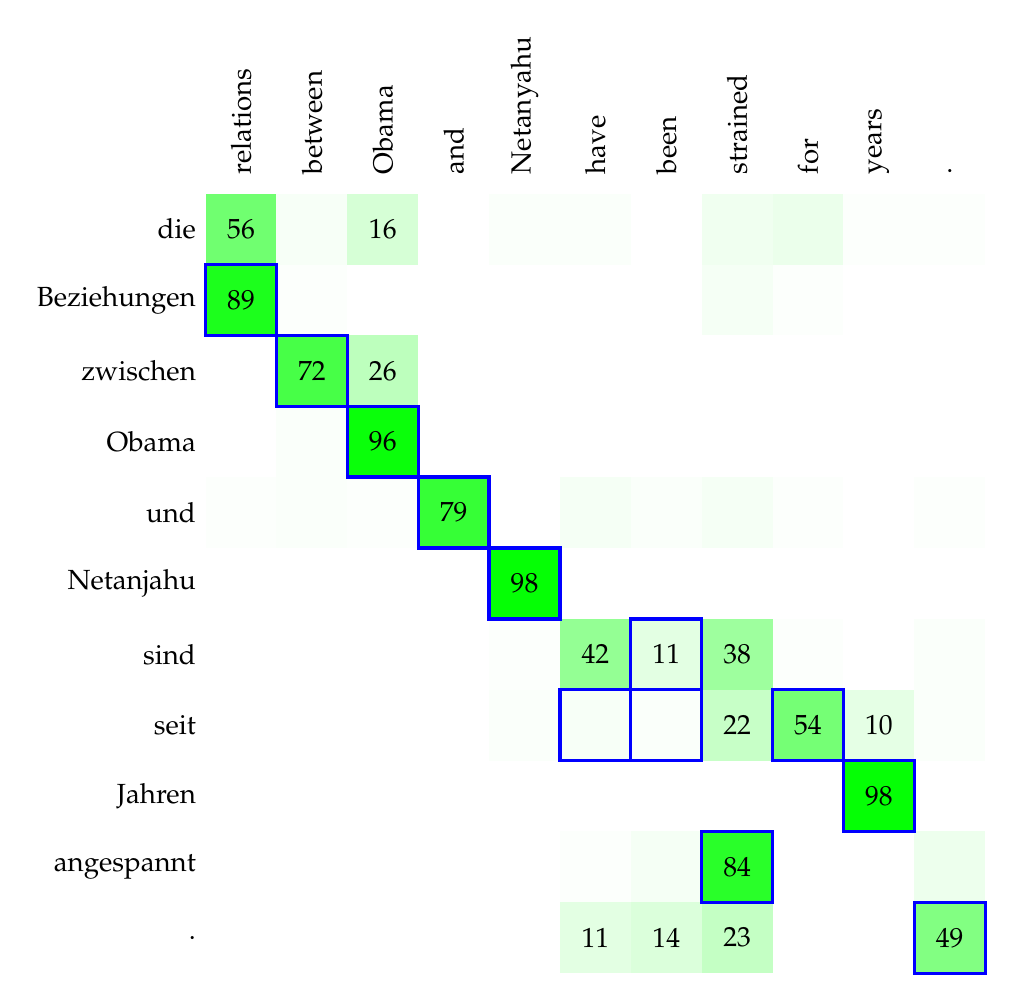
\begin{tikzpicture}[scale=0.9]
\node[label=above:\rotatebox{90}{relations}] at (0.5,11) {};
\node[label=above:\rotatebox{90}{between}] at (1.5,11) {};
\node[label=above:\rotatebox{90}{Obama}] at (2.5,11) {};
\node[label=above:\rotatebox{90}{and}] at (3.5,11) {};
\node[label=above:\rotatebox{90}{Netanyahu}] at (4.5,11) {};
\node[label=above:\rotatebox{90}{have}] at (5.5,11) {};
\node[label=above:\rotatebox{90}{been}] at (6.5,11) {};
\node[label=above:\rotatebox{90}{strained}] at (7.5,11) {};
\node[label=above:\rotatebox{90}{for}] at (8.5,11) {};
\node[label=above:\rotatebox{90}{years}] at (9.5,11) {};
\node[label=above:\rotatebox{90}{.}] at (10.5,11) {};
\draw (0,10.5) node[anchor=east] {die};
\draw (0,9.5) node[anchor=east] {Beziehungen};
\draw (0,8.5) node[anchor=east] {zwischen};
\draw (0,7.5) node[anchor=east] {Obama};
\draw (0,6.5) node[anchor=east] {und};
\draw (0,5.5) node[anchor=east] {Netanjahu};
\draw (0,4.5) node[anchor=east] {sind};
\draw (0,3.5) node[anchor=east] {seit};
\draw (0,2.5) node[anchor=east] {Jahren};
\draw (0,1.5) node[anchor=east] {angespannt};
\draw (0,0.5) node[anchor=east] {.};
\fill[green!56!white] (0,10) rectangle (1,11);
\draw (0.5,10.5) node[align=center] {56};
\fill[green!89!white] (0,9) rectangle (1,10);
\draw (0.5,9.5) node[align=center] {89};
\fill[green!0!white] (0,8) rectangle (1,9);
\fill[green!0!white] (0,7) rectangle (1,8);
\fill[green!1!white] (0,6) rectangle (1,7);
\fill[green!0!white] (0,5) rectangle (1,6);
\fill[green!0!white] (0,4) rectangle (1,5);
\fill[green!0!white] (0,3) rectangle (1,4);
\fill[green!0!white] (0,2) rectangle (1,3);
\fill[green!0!white] (0,1) rectangle (1,2);
\fill[green!0!white] (0,0) rectangle (1,1);
\fill[green!3!white] (1,10) rectangle (2,11);
\fill[green!1!white] (1,9) rectangle (2,10);
\fill[green!72!white] (1,8) rectangle (2,9);
\draw (1.5,8.5) node[align=center] {72};
\fill[green!2!white] (1,7) rectangle (2,8);
\fill[green!2!white] (1,6) rectangle (2,7);
\fill[green!0!white] (1,5) rectangle (2,6);
\fill[green!0!white] (1,4) rectangle (2,5);
\fill[green!0!white] (1,3) rectangle (2,4);
\fill[green!0!white] (1,2) rectangle (2,3);
\fill[green!0!white] (1,1) rectangle (2,2);
\fill[green!0!white] (1,0) rectangle (2,1);
\fill[green!16!white] (2,10) rectangle (3,11);
\draw (2.5,10.5) node[align=center] {16};
\fill[green!0!white] (2,9) rectangle (3,10);
\fill[green!26!white] (2,8) rectangle (3,9);
\draw (2.5,8.5) node[align=center] {26};
\fill[green!96!white] (2,7) rectangle (3,8);
\draw (2.5,7.5) node[align=center] {96};
\fill[green!1!white] (2,6) rectangle (3,7);
\fill[green!0!white] (2,5) rectangle (3,6);
\fill[green!0!white] (2,4) rectangle (3,5);
\fill[green!0!white] (2,3) rectangle (3,4);
\fill[green!0!white] (2,2) rectangle (3,3);
\fill[green!0!white] (2,1) rectangle (3,2);
\fill[green!0!white] (2,0) rectangle (3,1);
\fill[green!0!white] (3,10) rectangle (4,11);
\fill[green!0!white] (3,9) rectangle (4,10);
\fill[green!0!white] (3,8) rectangle (4,9);
\fill[green!0!white] (3,7) rectangle (4,8);
\fill[green!79!white] (3,6) rectangle (4,7);
\draw (3.5,6.5) node[align=center] {79};
\fill[green!0!white] (3,5) rectangle (4,6);
\fill[green!0!white] (3,4) rectangle (4,5);
\fill[green!0!white] (3,3) rectangle (4,4);
\fill[green!0!white] (3,2) rectangle (4,3);
\fill[green!0!white] (3,1) rectangle (4,2);
\fill[green!0!white] (3,0) rectangle (4,1);
\fill[green!2!white] (4,10) rectangle (5,11);
\fill[green!0!white] (4,9) rectangle (5,10);
\fill[green!0!white] (4,8) rectangle (5,9);
\fill[green!0!white] (4,7) rectangle (5,8);
\fill[green!0!white] (4,6) rectangle (5,7);
\fill[green!98!white] (4,5) rectangle (5,6);
\draw (4.5,5.5) node[align=center] {98};
\fill[green!1!white] (4,4) rectangle (5,5);
\fill[green!2!white] (4,3) rectangle (5,4);
\fill[green!0!white] (4,2) rectangle (5,3);
\fill[green!0!white] (4,1) rectangle (5,2);
\fill[green!0!white] (4,0) rectangle (5,1);
\fill[green!2!white] (5,10) rectangle (6,11);
\fill[green!0!white] (5,9) rectangle (6,10);
\fill[green!0!white] (5,8) rectangle (6,9);
\fill[green!0!white] (5,7) rectangle (6,8);
\fill[green!4!white] (5,6) rectangle (6,7);
\fill[green!0!white] (5,5) rectangle (6,6);
\fill[green!42!white] (5,4) rectangle (6,5);
\draw (5.5,4.5) node[align=center] {42};
\fill[green!3!white] (5,3) rectangle (6,4);
\fill[green!0!white] (5,2) rectangle (6,3);
\fill[green!1!white] (5,1) rectangle (6,2);
\fill[green!11!white] (5,0) rectangle (6,1);
\draw (5.5,0.5) node[align=center] {11};
\fill[green!0!white] (6,10) rectangle (7,11);
\fill[green!0!white] (6,9) rectangle (7,10);
\fill[green!0!white] (6,8) rectangle (7,9);
\fill[green!0!white] (6,7) rectangle (7,8);
\fill[green!2!white] (6,6) rectangle (7,7);
\fill[green!0!white] (6,5) rectangle (7,6);
\fill[green!11!white] (6,4) rectangle (7,5);
\draw (6.5,4.5) node[align=center] {11};
\fill[green!2!white] (6,3) rectangle (7,4);
\fill[green!0!white] (6,2) rectangle (7,3);
\fill[green!4!white] (6,1) rectangle (7,2);
\fill[green!14!white] (6,0) rectangle (7,1);
\draw (6.5,0.5) node[align=center] {14};
\fill[green!6!white] (7,10) rectangle (8,11);
\fill[green!4!white] (7,9) rectangle (8,10);
\fill[green!0!white] (7,8) rectangle (8,9);
\fill[green!0!white] (7,7) rectangle (8,8);
\fill[green!4!white] (7,6) rectangle (8,7);
\fill[green!0!white] (7,5) rectangle (8,6);
\fill[green!38!white] (7,4) rectangle (8,5);
\draw (7.5,4.5) node[align=center] {38};
\fill[green!22!white] (7,3) rectangle (8,4);
\draw (7.5,3.5) node[align=center] {22};
\fill[green!0!white] (7,2) rectangle (8,3);
\fill[green!84!white] (7,1) rectangle (8,2);
\draw (7.5,1.5) node[align=center] {84};
\fill[green!23!white] (7,0) rectangle (8,1);
\draw (7.5,0.5) node[align=center] {23};
\fill[green!8!white] (8,10) rectangle (9,11);
\fill[green!1!white] (8,9) rectangle (9,10);
\fill[green!0!white] (8,8) rectangle (9,9);
\fill[green!0!white] (8,7) rectangle (9,8);
\fill[green!1!white] (8,6) rectangle (9,7);
\fill[green!0!white] (8,5) rectangle (9,6);
\fill[green!1!white] (8,4) rectangle (9,5);
\fill[green!54!white] (8,3) rectangle (9,4);
\draw (8.5,3.5) node[align=center] {54};
\fill[green!0!white] (8,2) rectangle (9,3);
\fill[green!0!white] (8,1) rectangle (9,2);
\fill[green!0!white] (8,0) rectangle (9,1);
\fill[green!1!white] (9,10) rectangle (10,11);
\fill[green!0!white] (9,9) rectangle (10,10);
\fill[green!0!white] (9,8) rectangle (10,9);
\fill[green!0!white] (9,7) rectangle (10,8);
\fill[green!0!white] (9,6) rectangle (10,7);
\fill[green!0!white] (9,5) rectangle (10,6);
\fill[green!0!white] (9,4) rectangle (10,5);
\fill[green!10!white] (9,3) rectangle (10,4);
\draw (9.5,3.5) node[align=center] {10};
\fill[green!98!white] (9,2) rectangle (10,3);
\draw (9.5,2.5) node[align=center] {98};
\fill[green!0!white] (9,1) rectangle (10,2);
\fill[green!0!white] (9,0) rectangle (10,1);
\fill[green!1!white] (10,10) rectangle (11,11);
\fill[green!0!white] (10,9) rectangle (11,10);
\fill[green!0!white] (10,8) rectangle (11,9);
\fill[green!0!white] (10,7) rectangle (11,8);
\fill[green!1!white] (10,6) rectangle (11,7);
\fill[green!0!white] (10,5) rectangle (11,6);
\fill[green!2!white] (10,4) rectangle (11,5);
\fill[green!2!white] (10,3) rectangle (11,4);
\fill[green!0!white] (10,2) rectangle (11,3);
\fill[green!7!white] (10,1) rectangle (11,2);
\fill[green!49!white] (10,0) rectangle (11,1);
\draw (10.5,0.5) node[align=center] {49};
\draw[blue,very thick] (0,9) rectangle (1,10);
\draw[blue,very thick] (1,8) rectangle (2,9);
\draw[blue,very thick] (2,7) rectangle (3,8);
\draw[blue,very thick] (3,6) rectangle (4,7);
\draw[blue,very thick] (4,5) rectangle (5,6);
\draw[blue,very thick] (5,3) rectangle (6,4);
\draw[blue,very thick] (6,4) rectangle (7,5);
\draw[blue,very thick] (6,3) rectangle (7,4);
\draw[blue,very thick] (7,1) rectangle (8,2);
\draw[blue,very thick] (8,3) rectangle (9,4);
\draw[blue,very thick] (9,2) rectangle (10,3);
\draw[blue,very thick] (10,0) rectangle (11,1);
\end{tikzpicture}
\end{center}
\vfill

%%%%%%%%%%%%%%%%%%%%%%%%%%%%%%%%%%%%%%%%%%%%%%%%%%%%%%%%%%%%%%%%%%%%%%%%%%%%

\slide{Word Alignment?}
\vfill
\begin{center}
\small
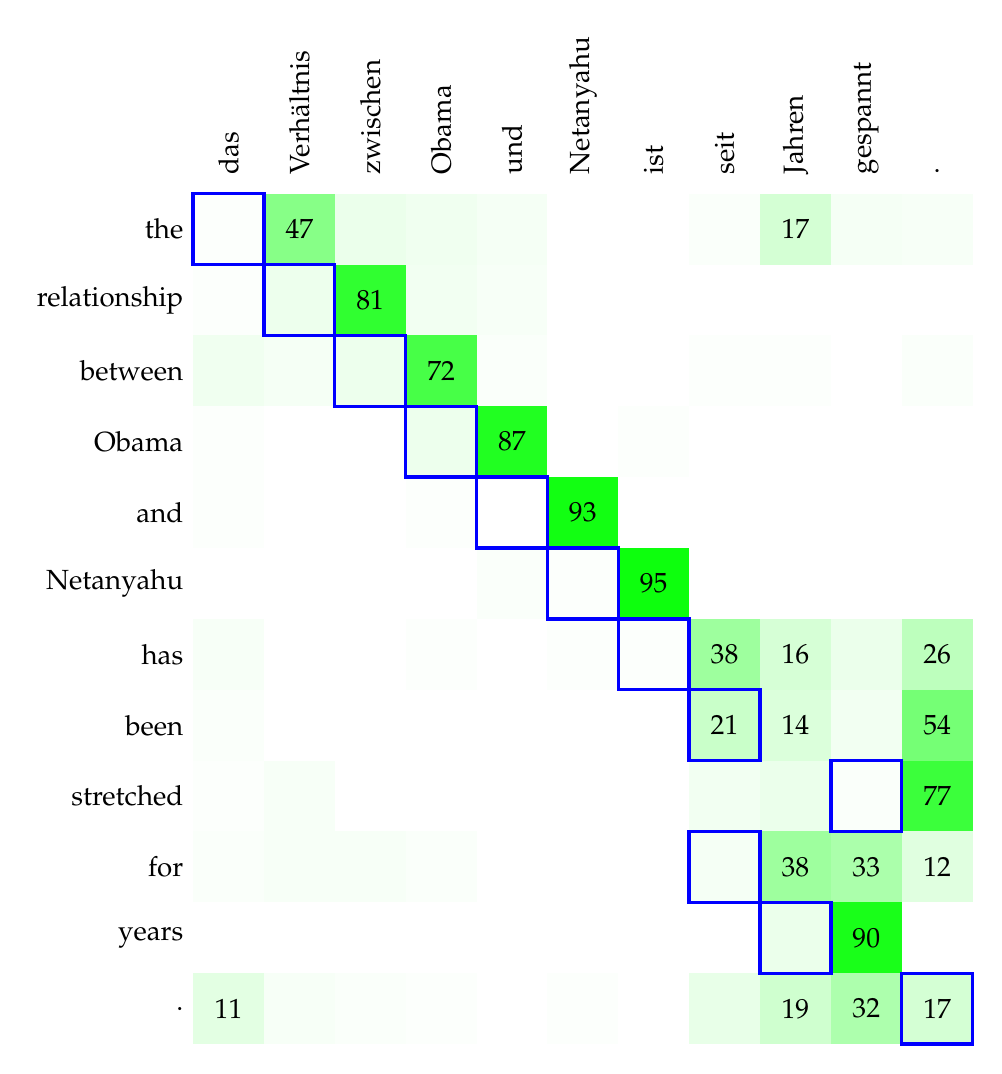
\begin{tikzpicture}[scale=0.9]
\node[label=above:\rotatebox{90}{das}] at (0.5,12) {};
\node[label=above:\rotatebox{90}{Verh\"altnis}] at (1.5,12) {};
\node[label=above:\rotatebox{90}{zwischen}] at (2.5,12) {};
\node[label=above:\rotatebox{90}{Obama}] at (3.5,12) {};
\node[label=above:\rotatebox{90}{und}] at (4.5,12) {};
\node[label=above:\rotatebox{90}{Netanyahu}] at (5.5,12) {};
\node[label=above:\rotatebox{90}{ist}] at (6.5,12) {};
\node[label=above:\rotatebox{90}{seit}] at (7.5,12) {};
\node[label=above:\rotatebox{90}{Jahren}] at (8.5,12) {};
\node[label=above:\rotatebox{90}{gespannt}] at (9.5,12) {};
\node[label=above:\rotatebox{90}{.}] at (10.5,12) {};
\draw (0,11.5) node[anchor=east] {the};
\draw (0,10.5) node[anchor=east] {relationship};
\draw (0,9.5) node[anchor=east] {between};
\draw (0,8.5) node[anchor=east] {Obama};
\draw (0,7.5) node[anchor=east] {and};
\draw (0,6.5) node[anchor=east] {Netanyahu};
\draw (0,5.5) node[anchor=east] {has};
\draw (0,4.5) node[anchor=east] {been};
\draw (0,3.5) node[anchor=east] {stretched};
\draw (0,2.5) node[anchor=east] {for};
\draw (0,1.5) node[anchor=east] {years};
\draw (0,0.5) node[anchor=east] {.};
\fill[green!1!white] (0,11) rectangle (1,12);
\fill[green!1!white] (0,10) rectangle (1,11);
\fill[green!6!white] (0,9) rectangle (1,10);
\fill[green!1!white] (0,8) rectangle (1,9);
\fill[green!1!white] (0,7) rectangle (1,8);
\fill[green!0!white] (0,6) rectangle (1,7);
\fill[green!3!white] (0,5) rectangle (1,6);
\fill[green!2!white] (0,4) rectangle (1,5);
\fill[green!1!white] (0,3) rectangle (1,4);
\fill[green!2!white] (0,2) rectangle (1,3);
\fill[green!0!white] (0,1) rectangle (1,2);
\fill[green!11!white] (0,0) rectangle (1,1);
\draw (0.5,0.5) node[align=center] {11};
\fill[green!47!white] (1,11) rectangle (2,12);
\draw (1.5,11.5) node[align=center] {47};
\fill[green!7!white] (1,10) rectangle (2,11);
\fill[green!4!white] (1,9) rectangle (2,10);
\fill[green!0!white] (1,8) rectangle (2,9);
\fill[green!0!white] (1,7) rectangle (2,8);
\fill[green!0!white] (1,6) rectangle (2,7);
\fill[green!0!white] (1,5) rectangle (2,6);
\fill[green!0!white] (1,4) rectangle (2,5);
\fill[green!3!white] (1,3) rectangle (2,4);
\fill[green!3!white] (1,2) rectangle (2,3);
\fill[green!0!white] (1,1) rectangle (2,2);
\fill[green!3!white] (1,0) rectangle (2,1);
\fill[green!8!white] (2,11) rectangle (3,12);
\fill[green!81!white] (2,10) rectangle (3,11);
\draw (2.5,10.5) node[align=center] {81};
\fill[green!7!white] (2,9) rectangle (3,10);
\fill[green!0!white] (2,8) rectangle (3,9);
\fill[green!0!white] (2,7) rectangle (3,8);
\fill[green!0!white] (2,6) rectangle (3,7);
\fill[green!0!white] (2,5) rectangle (3,6);
\fill[green!0!white] (2,4) rectangle (3,5);
\fill[green!0!white] (2,3) rectangle (3,4);
\fill[green!3!white] (2,2) rectangle (3,3);
\fill[green!0!white] (2,1) rectangle (3,2);
\fill[green!2!white] (2,0) rectangle (3,1);
\fill[green!6!white] (3,11) rectangle (4,12);
\fill[green!5!white] (3,10) rectangle (4,11);
\fill[green!72!white] (3,9) rectangle (4,10);
\draw (3.5,9.5) node[align=center] {72};
\fill[green!7!white] (3,8) rectangle (4,9);
\fill[green!1!white] (3,7) rectangle (4,8);
\fill[green!0!white] (3,6) rectangle (4,7);
\fill[green!1!white] (3,5) rectangle (4,6);
\fill[green!0!white] (3,4) rectangle (4,5);
\fill[green!0!white] (3,3) rectangle (4,4);
\fill[green!2!white] (3,2) rectangle (4,3);
\fill[green!0!white] (3,1) rectangle (4,2);
\fill[green!1!white] (3,0) rectangle (4,1);
\fill[green!4!white] (4,11) rectangle (5,12);
\fill[green!3!white] (4,10) rectangle (5,11);
\fill[green!2!white] (4,9) rectangle (5,10);
\fill[green!87!white] (4,8) rectangle (5,9);
\draw (4.5,8.5) node[align=center] {87};
\fill[green!0!white] (4,7) rectangle (5,8);
\fill[green!2!white] (4,6) rectangle (5,7);
\fill[green!0!white] (4,5) rectangle (5,6);
\fill[green!0!white] (4,4) rectangle (5,5);
\fill[green!0!white] (4,3) rectangle (5,4);
\fill[green!0!white] (4,2) rectangle (5,3);
\fill[green!0!white] (4,1) rectangle (5,2);
\fill[green!0!white] (4,0) rectangle (5,1);
\fill[green!0!white] (5,11) rectangle (6,12);
\fill[green!0!white] (5,10) rectangle (6,11);
\fill[green!0!white] (5,9) rectangle (6,10);
\fill[green!0!white] (5,8) rectangle (6,9);
\fill[green!93!white] (5,7) rectangle (6,8);
\draw (5.5,7.5) node[align=center] {93};
\fill[green!1!white] (5,6) rectangle (6,7);
\fill[green!1!white] (5,5) rectangle (6,6);
\fill[green!0!white] (5,4) rectangle (6,5);
\fill[green!0!white] (5,3) rectangle (6,4);
\fill[green!0!white] (5,2) rectangle (6,3);
\fill[green!0!white] (5,1) rectangle (6,2);
\fill[green!1!white] (5,0) rectangle (6,1);
\fill[green!0!white] (6,11) rectangle (7,12);
\fill[green!0!white] (6,10) rectangle (7,11);
\fill[green!0!white] (6,9) rectangle (7,10);
\fill[green!1!white] (6,8) rectangle (7,9);
\fill[green!0!white] (6,7) rectangle (7,8);
\fill[green!95!white] (6,6) rectangle (7,7);
\draw (6.5,6.5) node[align=center] {95};
\fill[green!1!white] (6,5) rectangle (7,6);
\fill[green!0!white] (6,4) rectangle (7,5);
\fill[green!0!white] (6,3) rectangle (7,4);
\fill[green!0!white] (6,2) rectangle (7,3);
\fill[green!0!white] (6,1) rectangle (7,2);
\fill[green!0!white] (6,0) rectangle (7,1);
\fill[green!2!white] (7,11) rectangle (8,12);
\fill[green!0!white] (7,10) rectangle (8,11);
\fill[green!1!white] (7,9) rectangle (8,10);
\fill[green!0!white] (7,8) rectangle (8,9);
\fill[green!0!white] (7,7) rectangle (8,8);
\fill[green!0!white] (7,6) rectangle (8,7);
\fill[green!38!white] (7,5) rectangle (8,6);
\draw (7.5,5.5) node[align=center] {38};
\fill[green!21!white] (7,4) rectangle (8,5);
\draw (7.5,4.5) node[align=center] {21};
\fill[green!5!white] (7,3) rectangle (8,4);
\fill[green!4!white] (7,2) rectangle (8,3);
\fill[green!0!white] (7,1) rectangle (8,2);
\fill[green!9!white] (7,0) rectangle (8,1);
\fill[green!17!white] (8,11) rectangle (9,12);
\draw (8.5,11.5) node[align=center] {17};
\fill[green!0!white] (8,10) rectangle (9,11);
\fill[green!1!white] (8,9) rectangle (9,10);
\fill[green!0!white] (8,8) rectangle (9,9);
\fill[green!0!white] (8,7) rectangle (9,8);
\fill[green!0!white] (8,6) rectangle (9,7);
\fill[green!16!white] (8,5) rectangle (9,6);
\draw (8.5,5.5) node[align=center] {16};
\fill[green!14!white] (8,4) rectangle (9,5);
\draw (8.5,4.5) node[align=center] {14};
\fill[green!8!white] (8,3) rectangle (9,4);
\fill[green!38!white] (8,2) rectangle (9,3);
\draw (8.5,2.5) node[align=center] {38};
\fill[green!8!white] (8,1) rectangle (9,2);
\fill[green!19!white] (8,0) rectangle (9,1);
\draw (8.5,0.5) node[align=center] {19};
\fill[green!4!white] (9,11) rectangle (10,12);
\fill[green!0!white] (9,10) rectangle (10,11);
\fill[green!0!white] (9,9) rectangle (10,10);
\fill[green!0!white] (9,8) rectangle (10,9);
\fill[green!0!white] (9,7) rectangle (10,8);
\fill[green!0!white] (9,6) rectangle (10,7);
\fill[green!8!white] (9,5) rectangle (10,6);
\fill[green!5!white] (9,4) rectangle (10,5);
\fill[green!2!white] (9,3) rectangle (10,4);
\fill[green!33!white] (9,2) rectangle (10,3);
\draw (9.5,2.5) node[align=center] {33};
\fill[green!90!white] (9,1) rectangle (10,2);
\draw (9.5,1.5) node[align=center] {90};
\fill[green!32!white] (9,0) rectangle (10,1);
\draw (9.5,0.5) node[align=center] {32};
\fill[green!3!white] (10,11) rectangle (11,12);
\fill[green!0!white] (10,10) rectangle (11,11);
\fill[green!2!white] (10,9) rectangle (11,10);
\fill[green!0!white] (10,8) rectangle (11,9);
\fill[green!0!white] (10,7) rectangle (11,8);
\fill[green!0!white] (10,6) rectangle (11,7);
\fill[green!26!white] (10,5) rectangle (11,6);
\draw (10.5,5.5) node[align=center] {26};
\fill[green!54!white] (10,4) rectangle (11,5);
\draw (10.5,4.5) node[align=center] {54};
\fill[green!77!white] (10,3) rectangle (11,4);
\draw (10.5,3.5) node[align=center] {77};
\fill[green!12!white] (10,2) rectangle (11,3);
\draw (10.5,2.5) node[align=center] {12};
\fill[green!0!white] (10,1) rectangle (11,2);
\fill[green!17!white] (10,0) rectangle (11,1);
\draw (10.5,0.5) node[align=center] {17};
\draw[blue,very thick] (0,11) rectangle (1,12);
\draw[blue,very thick] (1,10) rectangle (2,11);
\draw[blue,very thick] (2,9) rectangle (3,10);
\draw[blue,very thick] (3,8) rectangle (4,9);
\draw[blue,very thick] (4,7) rectangle (5,8);
\draw[blue,very thick] (5,6) rectangle (6,7);
\draw[blue,very thick] (6,5) rectangle (7,6);
\draw[blue,very thick] (7,4) rectangle (8,5);
\draw[blue,very thick] (7,2) rectangle (8,3);
\draw[blue,very thick] (8,1) rectangle (9,2);
\draw[blue,very thick] (9,3) rectangle (10,4);
\draw[blue,very thick] (10,0) rectangle (11,1);
\end{tikzpicture}
\end{center}
\vfill

%%%%%%%%%%%%%%%%%%%%%%%%%%%%%%%%%%%%%%%%%%%%%%%%%%%%%%%%%%%%%%%%%%%%%%%%%%%%

\slide{}
\vfill
\begin{center}
{\huge beam search}
\end{center}
\vfill

%%%%%%%%%%%%%%%%%%%%%%%%%%%%%%%%%%%%%%%%%%%%%%%%%%%%%%%%%%%%%%%%%%%%%%%%%%%%

\slide{Beam Search}
\vfill
\begin{center}
\begin{tikzpicture}
\begin{semilogxaxis}[
    xlabel={Beam Size},
    ylabel={BLEU},
    width=25cm,
    height=15cm,
    xmin=1, xmax=1000,
    ymin=28, ymax=31.5,
    xtick={1,2,4,8,12,20,30,50,100,200,500,1000},
    ytick={29,30,31},
    x tick label style={/pgf/number format/fixed},
    legend pos=south west,
    ymajorgrids=true,
    grid style=dashed,
    log base 10 number format code/.code={%
        $\pgfmathparse{int(10^(#1)+.5)}\pgfmathprintnumber{\pgfmathresult}$%
    }
]
    
%%% Unnormalized
\addplot[
    color=darkgreen,
    mark=o,
    nodes near coords,
    nodes near coords align={\thealign},
    visualization depends on={value \thisrow{ALIGN} \as \thealign},
    ]
    table[x=BEAM, y=BLEU]{
BEAM BLEU ALIGN
   1 29.7 south
   2 30.4 south
   4 30.5 south
   8 30.4 south
  12 30.3 south
  20 30.0 south
  30 29.8 south
  50 29.4 south
 100 28.5 south
 200 26.6 south
 500 21.7 south
1000 18.8 south
   };
    \addlegendentry{Unnormalized}
%%% Normalized
\addplot[
    color=green,
    mark=o,
    nodes near coords,
    nodes near coords align={\thealign},
    visualization depends on={value \thisrow{ALIGN} \as \thealign},
    ]
    table[x=BEAM, y=BLEU]{
BEAM BLEU ALIGN
   1 29.7 south
   2 30.4 south
   4 30.6 south
   8 30.8 south
  12 30.9 south
  20 30.9 south
  30 30.9 south
  50 30.9 south
 100 30.9 south
 200 30.7 south
 500 30.3 south
1000 29.9 south
    };
    \addlegendentry{Normalized}
\end{semilogxaxis}
\end{tikzpicture}
\end{center}
\vfill


%%%%%%%%%%%%%%%%%%%%%%%%%%%%%%%%%%%%%%%%%%%%%%%%%%%%%%%%%%%%%%%%%%%%%%%%%%%%

\slide{}
\vfill
\begin{center}
{\huge noisy data}
\end{center}
\vfill

%%%%%%%%%%%%%%%%%%%%%%%%%%%%%%%%%%%%%%%%%%%%%%%%%%%%%%%%%%%%%%%%%%%%%%%%%%%%

\slide{Noise in Training Data}
\vfill
\begin{itemize}\itemsep 1cm
\item Crawled parallel data from the web (very noisy)
\begin{center}
\begin{tabular}{l|c|c}
& \bf SMT & \bf NMT \\ \hline
WMT17 & 24.0 & 27.2 \\
+ Paracrawl & 25.2 (+1.2) & 17.3 (-9.9)\\
\end{tabular}

{\small (German-English, 90m words each of WMT17 and Crawl data)}

\includegraphics[scale=1]{noise-paracrawl.png}
\end{center}


\item Corpus cleaning methods \textcolor{purple}{[Xu and Koehn, EMNLP 2017]} give improvements
\end{itemize}
\vfill


%%%%%%%%%%%%%%%%%%%%%%%%%%%%%%%%%%%%%%%%%%%%%%%%%%%%%%%%%%%%%%%%%%%%%%%%%%%%

\slide{Types of Noise}
\vfill
\begin{itemize}
\item Misaligned sentences
\item Disfluent language (from MT, bad translations)
\item Wrong language data (e.g., French in German--English corpus)
\item Untranslated sentences
\item Short segments (e.g., dictionaries)
\item Mismatched domain
\end{itemize}
\vfill


%%%%%%%%%%%%%%%%%%%%%%%%%%%%%%%%%%%%%%%%%%%%%%%%%%%%%%%%%%%%%%%%%%%%%%%%%%%%

% for the next graphs

\newcommand{\debugcolor}{white}

\newcommand{\barchartnoise}[5]{\begin{tikzpicture}[scale=0.3]
\fill[\debugcolor] (5.7,0) rectangle (5.8,-#1);
\fill[\debugcolor] (5.7,0) rectangle (5.8,4);
\fill[green] (0,0) rectangle (5.5,0#3);
\fill[blue] (6,0) rectangle (11.5,0#5);
\draw (2.75,0) node[anchor=south] {#2};
\draw (8.75,0) node[anchor=south] {#4};
\draw (2.75,0#3) node[anchor=north] {\textcolor{red}{#3}};
\draw (8.75,0#5) node[anchor=north] {\textcolor{red}{#5}};
\end{tikzpicture}}

\newcommand{\positivebarchart}[5]{\begin{tikzpicture}[scale=0.3]
\fill[\debugcolor] (5.7,0) rectangle (5.8,-#1);
\fill[\debugcolor] (5.7,0) rectangle (5.8,4);
\fill[green] (0,0) rectangle (5.5,0#3);
\fill[blue] (6,0) rectangle (11.5,0#5);
\draw (2.75,0) node[anchor=south] {#2};
\draw (8.75,0) node[anchor=south] {#4};
\draw (2.75,0#3) node[anchor=north] {\textcolor{darkgreen}{#3}};
\draw (8.75,0#5) node[anchor=north] {\textcolor{darkgreen}{#5}};
\end{tikzpicture}}

\newcommand{\negposbarchart}[5]{\begin{tikzpicture}[scale=0.3]
\fill[\debugcolor] (5.7,0) rectangle (5.8,-#1);
\fill[\debugcolor] (5.7,0) rectangle (5.8,4);
\fill[green] (0,0) rectangle (5.5,0#3);
\fill[blue] (6,0) rectangle (11.5,0#5);
\draw (2.75,0) node[anchor=south] {#2};
\draw (8.75,0) node[anchor=south] {#4};
\draw (2.75,0#3) node[anchor=north] {\textcolor{red}{#3}};
\draw (8.75,0) node[anchor=north] {\textcolor{darkgreen}{#5}};
\end{tikzpicture}}

\newcommand{\rowlabelnoise}[2]{\begin{tikzpicture}[scale=0.15]
\fill[\debugcolor] (0,0) rectangle (0.1,4);
\fill[\debugcolor] (0,0) rectangle (0.1,-#1);
\draw (0,0) node[anchor=south] {\bf #2}; 
\end{tikzpicture}}

%%%%%%%%%%%%%%%%%%%%%%%%%%%%%%%%%%%%%%%%%%%%%%%%%%%%%%%%%%%%%%%%%%%%%%%%%%%%

\slide{Mismatched Sentences}
\vfill
\begin{itemize}
\item Artificial created by randomly shuffling sentence order
\item Added to existing parallel corpus in different amounts
\begin{center}
\begin{tabular}{c|c|c|c|c}
 \bf 5\% & \bf 10\%& \bf 20\%& \bf 50\%& \bf 100\% \\ \hline
    \barchartnoise{5.5}{    }{    }{24.0}{-0.0} & 
    \barchartnoise{5.5}{    }{    }{24.0}{-0.0} & 
    \barchartnoise{5.5}{    }{    }{23.9}{-0.1} & 
    \barchartnoise{5.5}{26.1}{-1.1}{23.9}{-0.1} & 
    \barchartnoise{5.5}{25.3}{-1.9}{23.4}{-0.6}\\\hline
\end{tabular}
\end{center}
\item Bigger impact on NMT (green, left) than SMT (blue, right)
\end{itemize}
\vfill

%%%%%%%%%%%%%%%%%%%%%%%%%%%%%%%%%%%%%%%%%%%%%%%%%%%%%%%%%%%%%%%%%%%%%%%%%%%%

\slide{Misordered Words}
\vfill
\begin{itemize}
\item Artificial created by randomly shuffling words in each sentence
\begin{center}
\begin{tabular}{l|c|c|c|c|c}
& \bf 5\% & \bf 10\%& \bf 20\%& \bf 50\%& \bf 100\% \\ \hline
\rowlabelnoise{5.5}{Source} & 
    \barchartnoise{5.5}{    }{    }{24.0}{-0.0} & 
    \barchartnoise{5.5}{    }{    }{23.6}{-0.4} & 
    \barchartnoise{5.5}{    }{    }{23.9}{-0.1} & 
    \barchartnoise{5.5}{26.6}{-0.6}{23.6}{-0.4} &
    \barchartnoise{5.5}{25.5}{-1.7}{23.7}{-0.3}\\
\rowlabelnoise{5.5}{Target} & 
    \barchartnoise{5.5}{    }{    }{24.0}{-0.0} & 
    \barchartnoise{5.5}{    }{    }{24.0}{-0.0} & 
    \barchartnoise{5.5}{    }{    }{23.4}{-0.6} & 
    \barchartnoise{5.5}{26.7}{-0.5}{23.2}{-0.8} &
    \barchartnoise{5.5}{26.1}{-1.1}{22.9}{-1.1}\\
\end{tabular}
\end{center}
\item Similar impact on NMT than SMT, worse for source reshuffle
\end{itemize}
\vfill

%%%%%%%%%%%%%%%%%%%%%%%%%%%%%%%%%%%%%%%%%%%%%%%%%%%%%%%%%%%%%%%%%%%%%%%%%%%%

\slide{Untranslated Sentences}
\vfill
\begin{center}
\begin{tabular}{l|c|c|c|c|c}
& \bf 5\% & \bf 10\%& \bf 20\%& \bf 50\%& \bf 100\% \\ \hline
\rowlabelnoise{28}{Source} & 
    \barchartnoise{28}{17.6}{ -9.8}{23.8}{-0.2} & 
    \barchartnoise{28}{11.2}{-16.0}{23.9}{-0.1} & 
    \barchartnoise{28}{ 5.6}{-21.6}{23.8}{-0.2} & 
    \barchartnoise{28}{ 3.2}{-24.0}{23.4}{-0.6} & 
    \barchartnoise{28}{ 3.2}{-24.0}{21.1}{-2.9}\\
\rowlabelnoise{5.5}{Target} & 
    \barchartnoise{5.5}{27.2}{-0.0}{    }{    } & 
    \barchartnoise{5.5}{27.0}{-0.2}{    }{    } & 
    \barchartnoise{5.5}{26.7}{-0.5}{    }{    } & 
    \barchartnoise{5.5}{26.8}{-0.4}{    }{    } &
    \barchartnoise{5.5}{26.9}{-0.3}{    }{    }\\ 
\end{tabular}
\end{center}
\vfill

%%%%%%%%%%%%%%%%%%%%%%%%%%%%%%%%%%%%%%%%%%%%%%%%%%%%%%%%%%%%%%%%%%%%%%%%%%%%

\slide{Wrong Language}
\vfill
\begin{center}
\begin{tabular}{l|c|c|c|c|c}
& \bf 5\% & \bf 10\%& \bf 20\%& \bf 50\%& \bf 100\% \\ \hline
\rowlabelnoise{5.5}{fr source} & 
    \barchartnoise{5.5}{26.9}{-0.3}{24.0}{-0.0} & 
    \barchartnoise{5.5}{26.8}{-0.4}{23.9}{-0.1} & 
    \barchartnoise{5.5}{26.8}{-0.4}{23.9}{-0.1} & 
    \barchartnoise{5.5}{26.8}{-0.4}{23.9}{-0.1} &
    \barchartnoise{5.5}{26.8}{-0.4}{23.8}{-0.2}\\
\rowlabelnoise{5.5}{fr target} & 
    \barchartnoise{5.5}{26.7}{-0.5}{24.0}{-0.0} & 
    \barchartnoise{5.5}{26.6}{-0.6}{23.9}{-0.1} & 
    \barchartnoise{5.5}{26.7}{-0.5}{23.8}{-0.2} & 
    \barchartnoise{5.5}{26.2}{-1.0}{23.5}{-0.5} &
    \barchartnoise{5.5}{25.0}{-2.2}{23.4}{-0.6}\\ \hline
\end{tabular}
\end{center}
\vfill
\begin{itemize}
\item Surprisingly robust, maybe due to domain mismatch of French data
\end{itemize}
\vfill

%%%%%%%%%%%%%%%%%%%%%%%%%%%%%%%%%%%%%%%%%%%%%%%%%%%%%%%%%%%%%%%%%%%%%%%%%%%%

\slide{Short Sentences}
\vfill
\begin{center}
\begin{tabular}{l|c|c|c|c}
& \bf 5\% & \bf 10\%& \bf 20\%& \bf 50\% \\ \hline
\rowlabelnoise{5.5}{1-2 words} & 
    \negposbarchart{5.5}{27.1}{-0.1}{24.1}{+0.1} & 
    \barchartnoise{5.5}{26.5}{-0.7}{23.9}{-0.1} & 
    \barchartnoise{5.5}{26.7}{-0.5}{23.8}{-0.2} &\\
\rowlabelnoise{5.5}{1-5 words} & 
    \positivebarchart{5.5}{27.8}{+0.6}{24.2}{+0.2} & 
    \positivebarchart{5.5}{27.6}{+0.4}{24.5}{+0.5} & 
    \positivebarchart{5.5}{28.0}{+0.8}{24.5}{+0.5} & 
    \negposbarchart{5.5}{26.6}{-0.6}{24.2}{+0.2} \\ \hline
\end{tabular}
\end{center}
\vfill
\begin{itemize}
\item No harm done
\end{itemize}
\vfill

%%%%%%%%%%%%%%%%%%%%%%%%%%%%%%%%%%%%%%%%%%%%%%%%%%%%%%%%%%%%%%%%%%%%%%%%%%%%

\slide{}
\vfill
\begin{center}
{\huge control over output}
\end{center}
\vfill

%%%%%%%%%%%%%%%%%%%%%%%%%%%%%%%%%%%%%%%%%%%%%%%%%%%%%%%%%%%%%%

\slide{Specifying Decoding Constraints}
\vfill
\begin{itemize}
\item Overriding the decisions of the decoder 
\item Why?
\begin{itemize}\itemsep 4mm
\item[$\Rightarrow$] translations have followed strict terminology
\item[$\Rightarrow$] rule-based translation of dates, quantities, etc.
\end{itemize}
\end{itemize}
\vfill

%%%%%%%%%%%%%%%%%%%%%%%%%%%%%%%%%%%%%%%%%%%%%%%%%%%%%%%%%%%%%%

\slide{XML Schema}
\vfill
\begin{center}\noindent
 \example{\em The} {\tt $<$x translation="Router"$>$}  \example{\em router} {\tt $<$/x$>$}  \example{\em is}  \tt{$<$wall/$>$}\\[3mm] 
  \example{\em a model} {\tt $<$zone$>$} \example{\em Psy X500 Pro} {\tt $<$/zone$>$}  \example{\em .}
\end{center}
\vfill
\begin{itemize}
\item The XML tags specify to the decoder that
\begin{itemize}\itemsep 3mm
\item the word \example{\em router} to be translated as \example{\em Router}
\item \example{\em The router is}, to be translated before the rest ({\tt <wall/>})
\item brand name \example{\em Psy X500 Pro} to be translated as a unit ({\tt <zone>, </zone>})
\end{itemize}
\end{itemize}
\vfill

%%%%%%%%%%%%%%%%%%%%%%%%%%%%%%%%%%%%%%%%%%%%%%%%%%%%%%%%%%%%%%%%%%%%%%%%%%%%

\slide{Formal Constraints}
\vfill
\begin{itemize}
\item Subtitles
\begin{itemize}
\item translation has to fit into space on screen\\ (may have to be shortened) 
\item input and output broken up into lines\pause
\end{itemize}
\item Speech translation
\begin{itemize}
\item input often not well-formed 
\item real time translation: start while sentence is spoken
\item subtitles: have be readable in limited time
\item dubbing: sync up with video of speaker's mouth movement\pause
\end{itemize}
\item Poetry
\begin{itemize}
\item meter
\item rhyme
\end{itemize}
\end{itemize}
\vfill

%%%%%%%%%%%%%%%%%%%%%%%%%%%%%%%%%%%%%%%%%%%%%%%%%%%%%%%%%%%%%%%%%%%%%%%%%%%%

\slide{}
\vfill
\begin{center}
{\huge questions?}
\end{center}
\vfill

\end{document}
